\documentclass[12pt,twoside, a4paper, twocolumn]{article}
\usepackage[utf8]{inputenc}
\usepackage[brazil]{babel}
\usepackage[margin = 0.5in]{geometry}
\usepackage{amsmath}
\usepackage{amsthm}
\usepackage{amssymb}
\usepackage{amsthm}
\usepackage{setspace}
\usepackage[americanvoltages,fulldiodes,siunitx]{circuitikz}
\usepackage{lipsum}
\usepackage{pgfplots}
\usepackage{ifthen}
\usepackage{adjustbox}
\usepackage[section]{placeins}
\usepackage{hyperref}
\usepackage{graphicx}
\usepackage{adjustbox}
\pgfplotsset{compat=newest}
\graphicspath{ {./images/} }
%  #1 color - optional #2 x_0 #3 y_0 #4 x_f #5 y_f #6 name - optional  #7 true if adding lines to axis
\newcommand{\drawvector} [9] [color=cyan] {
\draw[line width=1.5pt,#1,-stealth](axis cs: #2, #3)--(axis cs: #4, #5) node[anchor=south west]{$#6$};
\ifthenelse{\equal{#7}{true}}{
\draw[line width=1pt,#1, dashed](axis cs: #4, #5)--(axis cs: #4, 0) node[anchor= north west]{$#8$};
\draw[line width=1pt,#1, dashed](axis cs: #4, #5)--(axis cs: 0, #5) node[anchor=south east]{$#9$};
}
{}
}
\newcommand\deriv[2]{\frac{\mathrm d #1}{\mathrm d #2}}
\title{Sexto Relatório de Física Experimental 2}
\author{Henrique da Silva \\ hpsilva@proton.me}
\date{\today}
\pgfplotsset{width = 10cm, compat = 1.9}
\begin{document}
\maketitle
\pagenumbering{gobble}
\newpage
%pagenumbering{roman}
\tableofcontents
\newpage

\section{Introdução}

\paragraph*{Neste relatório, vamos discutir o funcionamento de um circuito $RC$, em particular suas funções como filtro e integrador de sinais de entrada.}


\section{Tarefas}

\subsection{Diagrama Fasorial}


\begin{adjustbox}{scale=0.9}
  \begin{tikzpicture}
    \begin{axis}[
      clip = false,
      xmin=0, xmax=2,
      ymin=0, ymax=2,
      axis lines=center,
      xlabel = $$, ylabel=$$,
      title={ },
      xtick={},
      xticklabels={}
      ytick={},
      yticklabels={}
      % xticklabel style = {anchor=south west},
      % xmajorgrids=true,
      % ymajorgrids=true,
      % grid style=dashed,
      ]


      % \addplot[domain=0:2*pi,color=blue, samples=100]{sin(deg(x))}
      % node[anchor=west, pos =0.7] {$3120$};



      \drawvector{0}{0}{1}{1}{V_{capacitor}}{true}{}{};
      \draw[line width=0pt,cyan,-stealth](axis cs: 0, 0)--(axis cs: 1, 1)  node[anchor= south east, pos =0.5] {};

      \draw [blue](axis cs: 0.0, 0.5) arc[start angle=90, end angle=45, radius=50]
      node[anchor= south west, pos =0.5] {$\phi$};

      \draw [blue](axis cs: 0.0, 0.3) arc[start angle=90, end angle=0, radius=30]
      node[anchor= south west, pos =0.2] {$wt$};


      \drawvector{0}{0}{-1}{1}{V_{resistor}}{true}{}{};
      \draw[line width=0pt,cyan,-stealth](axis cs: 0, 0)--(axis cs: -1, 1)  node[anchor= south west, pos =0.5] {};


      \drawvector{0}{0}{0}{1.41}{V_{entrada}}{true}{}{};
      \draw[line width=0pt,cyan,-stealth](axis cs: 0, 0)--(axis cs: 0, 1.41)  node[anchor= south east, pos =0.5] {};




    \end{axis}
  \end{tikzpicture}
\end{adjustbox}

\subparagraph*{Podemos daí tirar a conclusão de que as tensões no capacitor mais a tensão no resistor será apenas a decomposição vetorial da tensão de entrada. Logo segue:}

\begin{equation}
  \begin{aligned}
    V_{entrada}^2 & = V_{resistor}^2 + V_{capacitor}^2          \\
    V_{entrada}^2 & = (R*I_{entrada})^2 + (X_c * I_{entrada})^2 \\
    I_{entrada}   & = \frac{V_{entrada}}{\sqrt{R^2 + X_c^2}}    \\
  \end{aligned}
\end{equation}

\subparagraph*{Também temos a seguinte relação entre a voltagem, impedância e corrente no capacitor. Nao tenho certeza se por Lei de Ohm, mas por algo parecido que $V_c = I_m * X_c$. E como achamos uma função que descreve o I de entrada, ou seja, o $I_m$ acima. podemos então:}

\begin{equation}
  \begin{aligned}
    V_{c}         & = \frac{X_c V_m}{\sqrt{R^2 + X_c^2}}        \\
    V_{entrada}^2 & = (R*I_{entrada})^2 + (X_c * I_{entrada})^2 \\
    I_{entrada}   & = \frac{V_{entrada}}{\sqrt{R^2 + X_c^2}}    \\
  \end{aligned}
\end{equation}

\subparagraph*{Tambem temos que:}

\begin{equation}
  W_0 = \frac{1}{RC}
\end{equation}

\subparagraph*{Então finalmente substituindo acima:}

\begin{equation}
  \frac{V_{cm}}{V_{m}} = \frac{X_c}{\sqrt{1+ \frac{R^2}{X_c^2} }} = \frac{1}{1+ \sqrt{1+ \frac{R^2}{X_c^2} }} = \frac{1}{\sqrt{1+ \frac{w^2}{w_0^2}}}
\end{equation}

\subsection{Equações para impedancia, função transferência e ângulo de defasagem}

\subparagraph*{Impedancia: $\sqrt{R^2 + X_c^2}$}

\subparagraph*{Funcao de transferencia: $\frac{1}{\sqrt{1+ \frac{w^2}{w_0^2}}}$}

\subparagraph*{ ngulo de defasagem: $\arctan(\frac{w}{w_0})$ que no caso, e também claramente olhando pelo diagrama de fase será uma defasagem de $\frac{\pi}{4}$ em relação a tensão de entrada.}

\subsection{Tabela de dados}

\begin{center}
  \begin{tabular}{ |c|c|c|c| }
    \hline
    $F (Hz)$ & $ \frac{V_0}{V_e} (mV)$ & $\phi$ (graus) & $\phi$ (rad)           \\
             &                         &                &                        \\
    $50$     & $1 \pm 5 * 10^{-2}$     & $0 \pm 4$      & $0 \pm 3 * 10^{-2}$    \\
    $150$    & $0.97 \pm 5 * 10^{-2}$  & $13 \pm 4$     & $0.33 \pm 3 * 10^{-2}$ \\
    $250$    & $0.93 \pm 5 * 10^{-2}$  & $20 \pm 4$     & $0.35 \pm 3 * 10^{-2}$ \\
    $350$    & $0.88 \pm 5 * 10^{-2}$  & $30 \pm 4$     & $0.52 \pm 3 * 10^{-2}$ \\
    $400$    & $0.86 \pm 5 * 10^{-2}$  & $31 \pm 4$     & $0.55 \pm 3 * 10^{-2}$ \\
    $450$    & $0.87 \pm 5 * 10^{-2}$  & $32 \pm 4$     & $0.56 \pm 3 * 10^{-2}$ \\
    $500$    & $0.80 \pm 5 * 10^{-2}$  & $35 \pm 4$     & $0.61 \pm 3 * 10^{-2}$ \\
    $550$    & $0.81 \pm 5 * 10^{-2}$  & $40 \pm 4$     & $0.70 \pm 3 * 10^{-2}$ \\
    $600$    & $0.77 \pm 5 * 10^{-2}$  & $47 \pm 4$     & $0.73 \pm 3 * 10^{-2}$ \\
    $650$    & $0.75 \pm 5 * 10^{-2}$  & $45 \pm 4$     & $0.78 \pm 3 * 10^{-2}$ \\
    $700$    & $0.73 \pm 5 * 10^{-2}$  & $46 \pm 4$     & $0.80 \pm 3 * 10^{-2}$ \\
    $750$    & $0.7 \pm 5 * 10^{-2}$   & $48 \pm 4$     & $0.84 \pm 3 * 10^{-2}$ \\
    $800$    & $0.69 \pm 5 * 10^{-2}$  & $50 \pm 4$     & $0.87 \pm 3 * 10^{-2}$ \\
    $1000$   & $0.59 \pm 5 * 10^{-2}$  & $56 \pm 4$     & $0.98 \pm 3 * 10^{-2}$ \\
    $2000$   & $0.37 \pm 5 * 10^{-2}$  & $72 \pm 4$     & $1.26 \pm 3 * 10^{-2}$ \\
    $5000$   & $0.22 \pm 5 * 10^{-2}$  & $80 \pm 4$     & $1.40 \pm 3 * 10^{-2}$ \\
    $10000$  & $0.15 \pm 5 * 10^{-2}$  & $86 \pm 4$     & $1.50 \pm 3 * 10^{-2}$ \\
    $20000$  & $0.13 \pm 5 * 10^{-2}$  & $86 \pm 4$     & $1.50 \pm 3 * 10^{-2}$ \\
    $30000$  & $0.12 \pm 5 * 10^{-2}$  & $88 \pm 4$     & $1.53 \pm 3 * 10^{-2}$ \\
    $50000$  & $0.11 \pm 5 * 10^{-2}$  & $89 \pm 4$     & $1.55 \pm 3 * 10^{-2}$ \\

    \hline
  \end{tabular}
\end{center}

\subsection{Frequência de corte}

\subparagraph*{Achamos a frequência de corte em aproximadamente $700Hz$, mas poderia estar em qualquer frequencia entre $600$ e $800$ Hz.}

\subparagraph*{Apesar do $\frac{V_0}{V_e}$ para $750Hz$ estar mais próximo na tabela acima. Escolhemos o nosso valor de $700Hz$ por termos  mais confiança na defasagem de fase do que nas medições de $\frac{V_0}{V_e}$}

\subsection{Amplitude no resistor.}

\subparagraph*{Da equação (1) temos que $V_e^2 = V_c^2 + V_r^2$}

\subparagraph*{No caso da frequência de corte. a tensão no capacitor será $V_e*\frac{1}{\sqrt{2}}$}

\subparagraph*{Entao. $V_r = \sqrt{V_e^2 - \left(V_e*\frac{1}{\sqrt{2}}\right)^2 }$}

\subparagraph*{Vale notar também que para frequências de entrada baixas, a tensão do sistema inteiro estará no capacitor então $V_c = V_e$, e para frequências de entrada alta, a tensão inteira de entrada tenderá a estar no resistor então $V_r = V_e$}

\subsection{Gráficos}

\subparagraph*{No regime de alta frequências, se houver uma tensão de entrada de forma quadrada, veremos uma tensão triangular no capacitor.}

\subparagraph*{Se houver uma tensão triangular de entrada, veremos uma forma senoidal no capacitor.}

\subsubsection{Grafico para $V_e$ de forma quadrática}

\begin{adjustbox}{scale=0.5}

  \begin{tikzpicture}
    \begin{axis}[
        ylabel={Tensao },
        xlabel={Tempo },
        xmin = 0, xmax = 10,
        ymin = -6, ymax = 6.0,
        xtick distance = 2,
        ytick distance = 2,
        grid = both,
        minor tick num = 1,
        major grid style = {lightgray},
        minor grid style = {lightgray!25},
        width = 1\textwidth,
        height = 1\textwidth]
      \addplot[
        domain = 0:10,
        samples = 200,
        smooth,
        thick,
        blue,
      ] { 5*(2 / pi) * rad(asin(sin(deg(0.5*pi * \x))))};

    \end{axis}
  \end{tikzpicture}
\end{adjustbox}

\subsubsection{Grafico para $V_e$ de de forma triangular}

\begin{adjustbox}{scale=0.5}

  \begin{tikzpicture}
    \begin{axis}[
        ylabel={Tensao},
        xlabel={Tempo },
        xmin = 0, xmax = 10,
        ymin = -6, ymax = 6.0,
        xtick distance = 2,
        ytick distance = 2,
        grid = both,
        minor tick num = 1,
        major grid style = {lightgray},
        minor grid style = {lightgray!25},
        width = 1\textwidth,
        height = 1\textwidth]
      \addplot[
        domain = 0:10,
        samples = 200,
        smooth,
        thick,
        blue,
      ] { 4*(sin(deg(0.5*pi * \x)))};

    \end{axis}
  \end{tikzpicture}
\end{adjustbox}



\subsection{Filtro passa baixa e filtro passa alta}

\subparagraph*{Como discutido na seção 5, frequencias baixas terao sua tensão sendo "transferida" para a tensão do capacitor, enquanto frequencias altas terão sua tensão sendo "transferida" para o resistor.}

\subparagraph*{Então se quisermos filtrar frequências altas, medimos a tensão do capacitor, se quisermos filtrar frequências baixas, medimos a tensão no resistor.}

\subsection{Graficos de $V_0/V_e$ e $\phi$ para frequências de entrada}

\begin{adjustbox}{scale=0.70}
  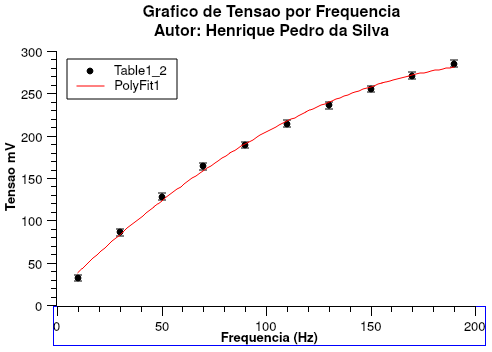
\includegraphics{Graph1.png}
\end{adjustbox}

\begin{adjustbox}{scale=0.70}
  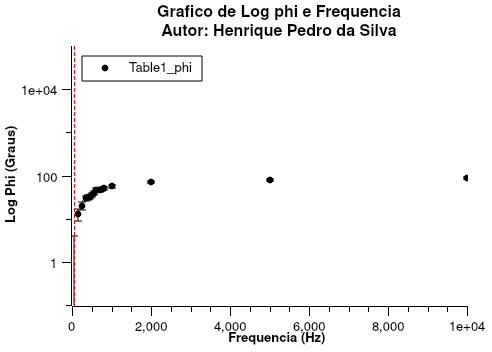
\includegraphics{Graph2.png}
\end{adjustbox}

\subparagraph*{Visualmente tive problemas para ver a frequência de corte. Mas fazendo o fit, obtive $734hz$.}




\end{document}